% THIS DOCUMENT IS TAILORED TO REQUIREMENTS FOR SCIENTIFIC COMPUTING.  IT SHOULDN'T
% BE USED FOR NON-SCIENTIFIC COMPUTING PROJECTS
\documentclass[12pt]{article}
\usepackage{svg}
\usepackage{hyperref}
\usepackage{amsmath, mathtools}
\usepackage{amsfonts}
\usepackage{amssymb}
\usepackage{graphicx}
\usepackage{colortbl}
\usepackage{xr}
\usepackage{hyperref}
\usepackage{longtable}
\usepackage{xfrac}
\usepackage{tabularx}
\usepackage{float}
\usepackage{siunitx}
\usepackage{booktabs}
\usepackage{caption}
\usepackage{pdflscape}
\usepackage{afterpage}
\usepackage{nameref}
\usepackage{enumitem}
\usepackage{lipsum}

\usepackage[round]{natbib}

\newlist{firstlinenoindent}{itemize}{1}

\setlist[firstlinenoindent]{itemindent=-\labelwidth}

%\usepackage{refcheck}

\hypersetup{
    bookmarks=true,         % show bookmarks bar?
      colorlinks=true,       % false: boxed links; true: colored links
    linkcolor=red,          % color of internal links (change box color with linkbordercolor)
    citecolor=green,        % color of links to bibliography
    filecolor=magenta,      % color of file links
    urlcolor=cyan           % color of external links
}

%% Comments

\usepackage{color}

\newif\ifcomments\commentstrue %displays comments
%\newif\ifcomments\commentsfalse %so that comments do not display

\ifcomments
\newcommand{\authornote}[3]{\textcolor{#1}{[#3 ---#2]}}
\newcommand{\todo}[1]{\textcolor{red}{[TODO: #1]}}
\newcommand{\note}[1]{\textcolor{red}{[#1 \#NOTE]}}
\else
\newcommand{\authornote}[3]{}
\newcommand{\todo}[1]{}
\fi

\newcommand{\wss}[1]{\authornote{blue}{SS}{#1}} 
\newcommand{\plt}[1]{\authornote{magenta}{TPLT}{#1}} %For explanation of the template
\newcommand{\an}[1]{\authornote{cyan}{Author}{#1}}


%% Common Parts


\newcommand{\progname}{Agolearn} % PUT YOUR PROGRAM NAME HERE
\newcommand{\thisproject}{\progname}
\newcommand{\authname}{Team 1, Agonaught(s)
\\ Yiding Li} % AUTHOR NAMES                  

\usepackage{hyperref}
    \hypersetup{colorlinks=true, linkcolor=blue, citecolor=blue, filecolor=blue,
                urlcolor=blue, unicode=false}
    \urlstyle{same}
                                


% For easy change of table widths
\newcommand{\colZwidth}{1.0\textwidth}
\newcommand{\colAwidth}{0.13\textwidth}
\newcommand{\colBwidth}{0.82\textwidth}
\newcommand{\colCwidth}{0.1\textwidth}
\newcommand{\colDwidth}{0.05\textwidth}
\newcommand{\colEwidth}{0.8\textwidth}
\newcommand{\colFwidth}{0.17\textwidth}
\newcommand{\colGwidth}{0.5\textwidth}
\newcommand{\colHwidth}{0.28\textwidth}

% Used so that cross-references have a meaningful prefix
\newcounter{defnum} %Definition Number
\newcommand{\dthedefnum}{GD\thedefnum}
\newcommand{\dref}[1]{GD\ref{#1}}
\newcounter{datadefnum} %Datadefinition Number
\newcommand{\ddthedatadefnum}{DD\thedatadefnum}
\newcommand{\ddref}[1]{DD\ref{#1}}
\newcounter{theorynum} %Theory Number
\newcommand{\tthetheorynum}{TM\thetheorynum}
\newcommand{\tref}[1]{TM\ref{#1}}
\newcounter{tablenum} %Table Number
\newcommand{\tbthetablenum}{TB\thetablenum}
\newcommand{\tbref}[1]{TB\ref{#1}}
\newcounter{scopnum} %Scope Decision Number
\newcommand{\athescopnumnum}{S\thescopnum}
\newcommand{\sref}[1]{S\ref{#1}}
\newcounter{assumpnum} %Assumption Number
\newcommand{\atheassumpnum}{A\theassumpnum}
\newcommand{\aref}[1]{A\ref{#1}}
\newcounter{goalnum} %Goal Number
\newcommand{\gthegoalnum}{GS\thegoalnum}
\newcommand{\gsref}[1]{GS\ref{#1}}
\newcounter{instnum} %Instance Number
\newcommand{\itheinstnum}{IM\theinstnum}
\newcommand{\iref}[1]{IM\ref{#1}}
\newcounter{reqnum} %Requirement Number
\newcommand{\rthereqnum}{R\thereqnum}
\newcommand{\rref}[1]{R\ref{#1}}
\newcounter{nfrnum} %NFR Number
\newcommand{\rthenfrnum}{NFR\thenfrnum}
\newcommand{\nfrref}[1]{NFR\ref{#1}}
\newcounter{lcnum} %Likely change number
\newcommand{\lthelcnum}{LC\thelcnum}
\newcommand{\lcref}[1]{LC\ref{#1}}

\newcommand*{\secref}[1]{\textbf{\hyperref[{#1}]{\ref*{#1} \nameref*{#1}}}}

\usepackage{fullpage}

\newcommand{\deftheory}[9][Not Applicable]
{
\newpage
\noindent \rule{\textwidth}{0.5mm}

\paragraph{RefName: } \textbf{#2} \phantomsection 
\label{#2}

\paragraph{Label:} #3

\noindent \rule{\textwidth}{0.5mm}

\paragraph{Equation:}

#4

\paragraph{Description:}

#5

\paragraph{Notes:}

#6

\paragraph{Source:}

#7

\paragraph{Ref.\ By:}

#8

\paragraph{Preconditions for \hyperref[#2]{#2}:}
\label{#2_precond}

#9

\paragraph{Derivation for \hyperref[#2]{#2}:}
\label{#2_deriv}

#1

\noindent \rule{\textwidth}{0.5mm}

}

\begin{document}


\title{Software Requirements Specification for \progname: An Evolutionary Black-Box Optimizer} 
\author{\authname}
\date{\today}
	
\maketitle

~\newpage

\pagenumbering{roman}

\tableofcontents

~\newpage

\section*{Revision History}

\begin{tabularx}{\textwidth}{p{3cm}p{2cm}X}
\toprule {\bf Date} & {\bf Version} & {\bf Notes}\\
\midrule
2024-01--22 & 0.1 & Initial draft\\
2024-02--02 & 0.2 & First complete draft\\
2024-02--02 & 0.2 & First coherent draft\\
\bottomrule
\end{tabularx}
This document is developed from a template based on \citet{SmithAndLai2005, SmithEtAl2007,
SmithAndKoothoor2016}. At the time of writing, this template is located at \href{https://github.com/smiths/capTemplate}{https://github.com/smiths/capTemplate}
~\\

~\newpage

\section{Reference Material}

This section records information for easy reference.

\subsection{Abbreviations and Acronyms}

\renewcommand{\arraystretch}{1.2}
\begin{tabular}{l l} 
  \toprule		
  \textbf{symbol} & \textbf{description}\\
  \midrule 
  A & Assumption\\
  DD & Data Definition\\
  GD & General Definition\\
  GS & Goal Statement\\
  IM & Instance Model\\
  LC & Likely Change\\
  PS & Physical System Description\\
  R & Requirement\\
  SRS & Software Requirements Specification\\
  \progname{} & Agnostic Learner\\
  TM & Theoretical Model\\
  \bottomrule
\end{tabular}\\

\subsection{Mathematical Notation}
\begin{tabular}{l l} 
  \toprule		
  \textbf{symbol} & \textbf{description}\\
  \midrule 
  $\mathbb{R}$ & Type of real numbers\\
  $\mathbb{R}^n$ & Type of real vectors\\
  $\mathbb{R}^n\rightarrow \mathbb{R}$ & Type of functions from real vectors to real numbers\\
  \bottomrule
\end{tabular}\\

\newpage

\pagenumbering{arabic}

\section{Introduction}

Black-box optimization problems deal with objective functions that are unknown, unexploitable, or non-existent\href{https://www.sciencedirect.com/science/article/pii/S2192440621001386}{ \textsuperscript{\textbf{*}}}.
As evolutionary algorithms lend well to optimizing against black-box objective functions, \thisproject{} seeks to implement an black-box optimizer using evolutionary methods.

This section includes the following subsections:
\begin{itemize}
  
  \item \secref{subsec:purpose}: A rough overview of this document: its intent, its contents, and its position in the development process.
  \item \secref{subsec:scopep}: Scope of problems that \thisproject{} seeks to address, an abstraction of assumptions.
  % \item \todo{The scope of the requirement is the scope of the project, in that we use the "faking it" process and are allowed to add requirements retroactively to the documention, so that the document serves as a reference, not just an artifact that we make then forget. So the requirement alwauys coverse the maximum of our knowledge and its scope extends to that of the project}
  \item \secref{subsec:reader}: Assumptions about the reader, including their knowledge and goals. This document is intended for readers who satisfy these assumptions.
  \item \secref{subsec:organ}: Major sections of this document that follow the introduction.
\end{itemize}

\subsection{Purpose of Document}
\label{subsec:purpose}

% There must be a better way to put it.
This document records requirement specifications of \progname{}, in particular of the software that should satisfy these requirements. This document explains requirement specifications in the following parts:

\begin{itemize}
  \item Scope and refined assumptions
  \item Problem and refined goals
  \item Theoretical foundation and refined models
  \item Inputs and outputs
  \item Functional and nonfunctional requirements
\end{itemize}

\subsection{Scope of Project} 
\label{subsec:scopep}
% Mention of Genomes precedes definitions, which are defined in 2.3 earliest.
Genomes, in particular variators that operate upon genomes, are costly to implement. As such, \thisproject{} only implements genomes of real vectors and genetic programs and only implements objective functions from these types. This scope decision refines to \aref{A_TYPE_REAL} and \aref{A_TYPE_HIGHER}
% Can I say "this scope decision ... refines to ... ?"
\thisproject{} use evolutionary algorithms, which are iterative, do not guarantee optimality, and do not incorporate hard constraints. This scope decision refines to \aref{A_ONLYEVO}, \aref{A_NOPOT}, \aref{A_ITER}, and \aref{A_NOCON}.

\thisproject{} is a library. This assumption removes the need to consider complex user interfaces. This scope decision refines to \aref{A_DAD_IM_A_LIBRARY}.

\subsection{Characteristics of Intended Reader} \label
{sec_IntendedReader}
\label{subsec:reader}

Readers of this document should have proficiency in at least high school level math\href{https://www.edu.gov.on.ca/eng/curriculum/secondary/math1112currb.pdf}{\textsuperscript{link}}. In addition, readers should be familiar with the following concepts relating to optimization and evolutionary learning:

\begin{itemize}
  \item Optimization: Objective functions, hyper-parameters, and iterative processes
  \item The balance between quality and novelty
  \item Evolutionary operators: (a) evaluator, (b) variator, (c) selectors, and their roles in the evolutionary process
\end{itemize}

Familiarity with terminologies defined in \secref{subsubsec:terms} are helpful, but not required to understand this document.

\subsection{Organization of Document}
\label{subsec:organ}

This document begins with an overview of this document and \thisproject, including: (a) the purpose of \thisproject, (b) the scope of \thisproject, and (c) characteristics of the intended reader.

Subsequent sections describes the system in increasing specificity, ending with a mathematical definitions of the system. These sections are:



\begin{firstlinenoindent}
% Descriptions are copied verbatim
\item[] \secref{sec:general}: General information about the system.  It identifies the interfaces between the system and its environment, describes the user characteristics and lists the system constraints.

\item[] \secref{sec:specific}: This section first presents the problem description, which gives a high-level
view of the problem to be solved.  This is followed by the solution characteristics
specification, which presents the assumptions, theories, definitions and finally
the instance models.

\item[] \secref{sec:requirements}: This section provides the functional requirements, the business tasks that the
software is expected to complete, and the nonfunctional requirements, the qualities that the software is expected to exhibit.

\item[] \secref{sec:lchanges} and \secref{sec:uchanges}: These sections document anticipated changes to requirements. This information instructs design and implementation.

% Requirement items?
\item[] \secref{sec:tracer}: This section connects requirement items in this document. Requirement items include (a) assumptions, (b) goal statements, (c) instance models, (d) functional requirements, (e) nonfunctional requirements, (f) likely changes, and (g) unlikely changes.

\end{firstlinenoindent}

\section{General System Description}
This section includes the following subsections:
\begin{itemize}
  \item \secref{subsec:syscontext}: Abstract interface and responsibilities of the software
  \item \secref{subsec:userchar}: Characteristics of expected users of the software
\end{itemize}
\label{sec:general}

\subsection{System Context}
\label{subsec:syscontext}

\thisproject implements an optimizer. As an optimizer, \thisproject takes (a) an objective function and (b) hyper-parameters that instruct the optimization process. As an optimizer, \thisproject outputs a solution that optimizes the given objective function. \autoref{Fig_SystemContext} describes the interaction between \thisproject and the user.

\begin{figure}[h!]
\begin{center}
 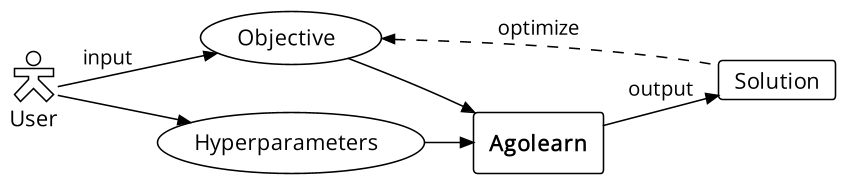
\includegraphics[width=0.8\textwidth]{agolearn}
\caption{System Context}
\label{Fig_SystemContext} 
\end{center}
\end{figure}

% In some systems, such as self driving cars,  responsibility extends beyond the system. For example, the user is responsible for following GPS navigation instructions to get to the destination.
Responsibilities of \thisproject and the user are as follows. Appropriate performance of \thisproject to its specification requires that both responsibilities are satisfied.
\begin{itemize}
  \item User Responsibility:
  \begin{itemize}
  \item Provide correctly typed inputs
  \end{itemize}
  \item \progname{} Responsibilities:
  \begin{itemize}
  \item Detect and report mistyped inputs
  \item Detect and report constraint violations of the input
  \item Calculate required outputs
  \end{itemize}
\end{itemize}

\subsection{User Characteristics} \label{SecUserCharacteristics}
\label{subsec:userchar}

The intended user of \thisproject{} has the following characteristics:

\begin{itemize}
  \item Motivation: The user seeks to optimize an objective function of real numbers or functions.
  \item Capability: The user can make function calls to libraries
  \item Capability: The user is familiarity with evolutionary operators and can choose from a pre-defined catalogue of operators.
\end{itemize}

\section{Specific System Description}
\label{sec:specific}

This section includes the following subsections:
\begin{itemize}
  \item \secref{subsec:problemdesc}: Description and refinements of the problem
  \item \secref{subsec:solchar}: Characteristics of a good solution, which \thisproject{} should produce
  \item \secref{subsec:scope}: Scope decisions that affect design and implementation
\end{itemize}


\subsection{Problem Description} \label{Sec_pd}
\label{subsec:problemdesc}

% Is this part necessary?
Optimization of black-box functions: functions that do not follow a particular form.

\subsubsection{Terminology and Definitions}
\label{subsubsec:terms}

% I consider moving them to earlier - or maybe it's better to move the terms that occur before to after this point.
The following terms are used in subsequent sections:

\begin{itemize}
  \item Genetic program: A evolutionary algorithm that generates genetic programs
  \item Genetic programming algorithm: A program that is evolutionarily produced
  \item Evolutionary operators: Operators that constitute a evolutionary algorithm
  \item Genome: A representation of a solution
  \item Evaluator: An evolutionary operator that evaluates the fitness of a genome
  \item Variator: An evolutionary operator that modifies genomes
  \item Selector: An evolutionary operator that selects from a pool of genomes
  \item Parents: A pool of genomes about to undergo variation
  \item Offspring: The output of a variator
  \item Fitness: The score of a genome according to the evaluator
\end{itemize}



\begin{figure}[h!]
	\begin{center}
		%\rotatebox{-90}
		{
			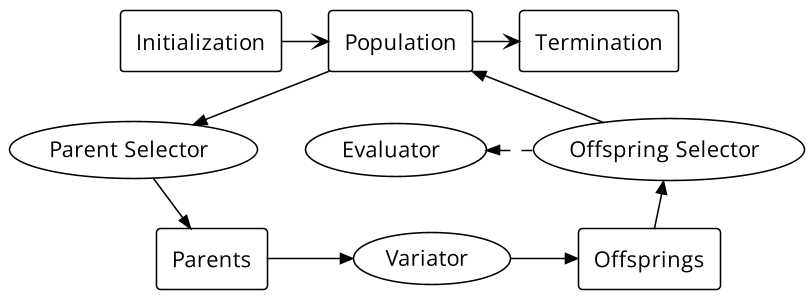
\includegraphics[width=0.8\textwidth]{pasta}
		}
		\caption{\label{fig:evoalg} Evolutionary Operators and their Positions in an Evolutionary Algorithm}
	\end{center}
\end{figure}


\subsubsection{Goal Statements}

\thisproject{} accepts objective function as evaluators. For each objective function, \thisproject{} returns a genome with optimal fitness.

\noindent In particular, given the assumed inputs, the goal statements are:

\begin{itemize}

\item[GS\refstepcounter{goalnum}\thegoalnum \label{GS_REALS}:] Optimize against real-valued functions
\item[GS\refstepcounter{goalnum}\thegoalnum \label{GS_HIGHER}:] Optimize against higher-order functions
% This reference to assumptions is anachronistic. Should assumptions come from all else, or should assumptions reference goals?
\end{itemize}

\subsection{Solution Characteristics Specification}
\label{subsec:solchar}

The output of \thisproject{} optimizes the given objective function. The solution should have the same type of the initial population.

The highest score of the output should be greater or equal to that of the initial population.


The instance models that govern \progname{} are presented in
Subsection~\ref{sec_instance}.  The information to understand the meaning of the
instance models and their derivation is also presented, so that the instance
models can be verified.

\subsection{Scope Decisions}
\label{subsec:scope}

This system only optimizes functions of real numbers, as well as higher-order functions.

An evolutionary algorithm must define a variator for each individual selector. Such variators are costly to implement and it would be difficult to require them as user inputs. The decision is made to restrict representations to two types: vectors of real values and higher-order functions. 

Consequently, the restriction on the types of solutions restricts the range of inputs


\subsubsection{Assumptions} \label{sec_assumpt}

\begin{itemize}

\item[A\refstepcounter{assumpnum}\theassumpnum \label{A_TYPE_REAL}:] The input objective function can be real-valued (\gsref{GS_REALS})
\item[A\refstepcounter{assumpnum}\theassumpnum \label{A_TYPE_HIGHER}:] The input objective function can be higher-ordered (\gsref{GS_HIGHER})
\item[A\refstepcounter{assumpnum}\theassumpnum \label{A_ONLYEVO}:] 
\thisproject{} implements evolutionary algorithms
% A better word for "... only implements"?
\item[A\refstepcounter{assumpnum}\theassumpnum \label{A_NOPOT}:] \thisproject{} may not output the global optimum of the input objective function.
\item[A\refstepcounter{assumpnum}\theassumpnum \label{A_ITER}:] \thisproject{} is an iterative optimizer.
\item[A\refstepcounter{assumpnum}\theassumpnum \label{A_NOCON}:] \thisproject{} does not accept explicit constraints.
\item[A\refstepcounter{assumpnum}\theassumpnum \label{A_DAD_IM_A_LIBRARY}:] \thisproject{} is a library.


\end{itemize}

\subsubsection{Instance Models} \label{sec_instance}    

The following instance models describe systems that corresponds to goals.

~\newline
\noindent
\begin{minipage}{\textwidth}
\renewcommand*{\arraystretch}{1.5}
\begin{tabular}{| p{\colAwidth} | p{\colBwidth}|}
  \hline
  \rowcolor[gray]{0.9}
  Number& IM\refstepcounter{instnum}\theinstnum \label{IM_REALS}\\
  \hline
  Label& \bf Optimize real-valued functions\\
  \hline
  Input&$F : \mathbb{R}^n\rightarrow \mathbb{R}$\\
  \hline
  Output&$X : \mathbb{R}^n$\\
  \hline
  Description&The system receives a real-valued objective function, then emits a real vector that optimizes the objective function. \\
  \hline
  Goal&\gsref{GS_REALS}
  \\
  \hline
\end{tabular}
\end{minipage}\\

~\newline
\noindent
\begin{minipage}{\textwidth}
\renewcommand*{\arraystretch}{1.5}
% I find it useful to move references to the matrix - otherwise the same information is repeated in two places.
\begin{tabular}{| p{\colAwidth} | p{\colBwidth}|}
  \hline
  \rowcolor[gray]{0.9}
  Number& IM\refstepcounter{instnum}\theinstnum \label{IM_HIGHER}\\
  \hline
  Label& \bf Optimize higher-order functions\\
  \hline
  Input&$F : (A^n\rightarrow B)\rightarrow \mathbb{R}$\\
  \hline
  Output&$X : (A^n\rightarrow B)$\\
  \hline
  Description&The system receives a higher-order objective function of functions, then emits a function that optimizes the given objective function.\\
  \hline
  Goal&\gsref{GS_HIGHER}
  \\
  \hline
\end{tabular}
\end{minipage}\\

%~\newline

\subsubsection{Properties of a Correct Solution} \label{sec_CorrectSolution}

\noindent

The output of \thisproject{} seeks, but not necessarily, optimize the input objective function (\aref{A_NOPOT}).

Because \thisproject{} is an iterative optimizer (\aref{A_ITER}), the best genome in each generation has a better fitness than the best genome in the last generation.

% This is incredibly verbose.

\section{Requirements}
\label{sec:requirements}

This section includes the following subsections:
\begin{itemize}
  \item \secref{subsubsec:freq}: Requirements that make explicit tasks and behaviours the software should complete
  \item \secref{subsubsec:nfreq}: Requirements that facilitate the satisfaction of functional requirements
  \item \secref{subsubsec:rationale}: Rationale for scope decisions, modeling decision, and assumptions
\end{itemize}

\subsection{Functional Requirements}
\label{subsubsec:freq}
\noindent \begin{itemize}
% I wonder if these two requirements may be helpful.
\item[R\refstepcounter{reqnum}\thereqnum \label{R_TYPECHECK}:] The system checks if input values are correctly typed and within input constraints.
\item[R\refstepcounter{reqnum}\thereqnum \label{R_TYPETHEN}:] If input values are correctly typed and within input constraints, then the system should operate normally (satisfy all requirements).

\item[R\refstepcounter{reqnum}\thereqnum \label{R_EVOCHANGE}:] Evolutionary operators of the same type can be used interchangeably 

\item[R\refstepcounter{reqnum}\thereqnum \label{R_IMBETTER}:] Each generation of the algorithm (\aref{A_ITER}) should produce a genome with equal or higher fitness than the previous generation (\aref{A_NOPOT}).

\end{itemize}

\subsection{Nonfunctional Requirements}
\label{subsubsec:nfreq}


\noindent \begin{itemize}

\item[NFR\refstepcounter{nfrnum}\thenfrnum \label{NFR_Accuracy}:]
  \textbf{Accuracy} Each iteration of the algorithm should produce a solution whose value, when given to the given objective function, is better than that of the best solution of the previous iteration.

\item[NFR\refstepcounter{nfrnum}\thenfrnum \label{NFR_Usability-Impl}:] \textbf{Usability-Implementation}
  The software should be implemented as a library and expose an interface in the form of function calls

  \item[NFR\refstepcounter{nfrnum}\thenfrnum \label{NFR_Usability}:] \textbf{Usability-Docs}
  Every public variables, functions, and class should be described.

\item[NFR\refstepcounter{nfrnum}\thenfrnum \label{NFR_Maintainability}:]
  \textbf{Maintainability} 
  Implementation of the software should be typed. Where types cannot be enforced, types must be hinted.

\item[NFR\refstepcounter{nfrnum}\thenfrnum \label{NFR_Portability}:]
  \textbf{Portability} The system should be able to run on Windows 11, up to 024-01 Cumulative Update for Windows 11 Version 22H2 for x64-based Systems (KB5034123)
  

\end{itemize}

\subsection{Rationale}
\label{subsubsec:rationale}

% Question here
\note{None at the moment}

\section{Likely Changes}
\label{sec:lchanges}

\noindent \begin{itemize}

\item[LC\refstepcounter{lcnum}\thelcnum\label{LC_EVOP}:] The selection of evolution operators have not been defined and will change.
\item[LC\refstepcounter{lcnum}\thelcnum\label{LC_HYPER}:] Hyper-parameters are not concretely defined. The types of hyperparameter inputs will change.
\item[LC\refstepcounter{lcnum}\thelcnum\label{LC_OBJC}:] Implementation of other types of objective functions.

\end{itemize}

\section{Unlikely Changes}   
\label{sec:uchanges} 

\noindent \begin{itemize}

\item[LC\refstepcounter{lcnum}\thelcnum\label{ULC_TECHNOLOGY}:] Implement \thisproject with another technology than evolutionary models

\item[LC\refstepcounter{lcnum}\thelcnum\label{ULC_FINDOPTIMUM}:] Add assurance that the result is a global optimum

\end{itemize}

\section{Traceability Matrices and Graphs}
\label{sec:tracer}

The purpose of the traceability matrices is to provide easy references on what
has to be additionally modified if a certain component is changed.  Every time a
component is changed, the items in the column of that component that are marked
% with an ``X'' may have to be modified as well.  Table~\ref{Table:trace} shows the
% dependencies of theoretical models, general definitions, data definitions, and
% instance models with each other. 
Table~\ref{Table:R_trace} shows the
dependencies of instance models, requirements, and data constraints on each
other. Table~\ref{Table:A_trace} shows the dependencies of theoretical models,
general definitions, data definitions, instance models, and likely changes on
the assumptions.

\afterpage{



\begin{landscape}
\begin{table}[h!]
\centering
\begin{tabular}{|c|c|c|c|c|c|c|c|c|c|c|c|c|c|c|c|c|c|c|c|}
\hline
& \gsref{GS_REALS}
& \gsref{GS_HIGHER}
& \rref{R_IMBETTER}
& \aref{A_NOPOT}
& \aref{A_ITER}\\

\hline
\aref{A_TYPE_REAL}        &$\leftarrow$& & & & \\
\aref{A_TYPE_HIGHER}      & &$\leftarrow$& & & \\
\aref{A_ONLYEVO}          & & & &$\rightarrow$&$\rightarrow$\\
\aref{A_NOPOT}            & & &$\rightarrow$& & \\
\aref{A_ITER}             & & &$\rightarrow$& & \\
\aref{A_NOCON}            & & & & & \\
\aref{A_DAD_IM_A_LIBRARY} & & & & & \\ 

\end{tabular}
\caption{Traceability Matrix Showing the Connections Between Assumptions and Other Items}
\label{Table:A_trace}
\end{table}

\begin{table}[h!]
  \centering
  \begin{tabular}{|c|c|c|c|c|c|c|c|}
  \hline
    & \iref{IM_REALS}& \iref{IM_HIGHER}\\
  \hline
  \aref{R_EVOCHANGE}             &X&X \\ \hline
  \aref{R_TYPETHEN}             & X&X \\ \hline
  \aref{R_TYPECHECK}             & X&X \\ \hline
  \aref{R_IMBETTER}             & X&X \\ \hline
  
  \hline
  \end{tabular}
  % Would it be better to connect goals and instance models?
  \caption{Traceability Matrix Showing the Connections Between Requirements and Instance Models}
  \label{Table:R_trace}
  \end{table}

  \begin{figure}[h!]
    \begin{center}
      {
        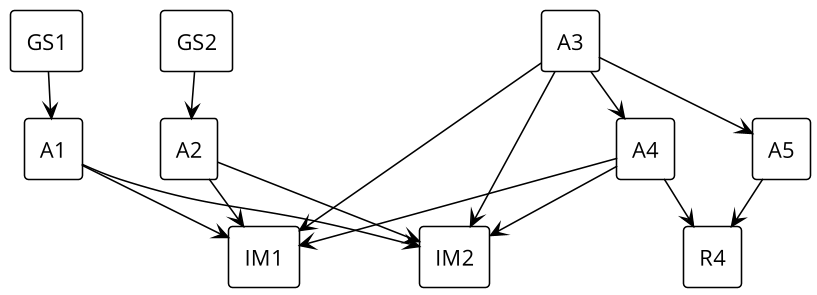
\includegraphics[width=0.7\textwidth]{goblin.png}
      }
      \caption{\label{Fig_RTrace} Traceability Matrix Showing the 
  Connections Between Assumptions, Goal Statements, and Instance Models}
    \end{center}
  \end{figure}

\end{landscape}
}

% \begin{table}[h!]
% \centering
% \begin{tabular}{|c|c|c|c|c|c|c|c|c|c|c|c|c|c|c|c|c|c|c|c|c|c|c|c|}
% \hline        
% 	& \tref{T_COE}& \tref{T_SHE}\\
% \hline
% \tref{T_COE}     & & \\ \hline
% \tref{T_SHE}     & & \\
% \hline
% \end{tabular}
% \caption{Traceability Matrix Showing the Connections Between Items of Different Sections}
% \label{Table:trace}
% \end{table}

The purpose of the traceability graphs is also to provide easy references on
what has to be additionally modified if a certain component is changed.  The
arrows in the graphs represent dependencies. The component at the tail of an
arrow is depended on by the component at the head of that arrow. Therefore, if a
component is changed, the components that it points to should also be
changed. 



% I do not have these things
%Figure~\ref{Fig_ATrace} shows the dependencies of theoretical models,
% general definitions, data definitions, instance models, likely changes, and
% assumptions on each other. Figure~\ref{Fig_RTrace} shows the dependencies of
% instance models, requirements, and data constraints on each other.

% \begin{figure}[h!]
% 	\begin{center}
% 		%\rotatebox{-90}
% 		{
% 			\includegraphics[width=\textwidth]{ATrace.png}
% 		}
% 		\caption{\label{Fig_ATrace} Traceability Matrix Showing the Connections Between Items of Different Sections}
% 	\end{center}
% \end{figure}












\section{Development Plan}

Develop an abstract framework that represents the evolutionary process, then craft instances of these operators.

\section{Values of Auxiliary Constants}

\note{None at the moment}


\newpage

\bibliographystyle {plainnat}
\bibliography {../../refs/References}

\newpage

\end{document}